\documentclass[titlepage]{article}
\usepackage{listings}
\usepackage[final]{pdfpages}

\lstset{%
  numbers=left,
  numberstyle=\tiny,
  basicstyle=\ttfamily,
  breaklines=true,
  frame=tb
}

\lstdefinestyle{CANSI}
{
    language=[Ansi]C,
    literate = *{\ \ }{}0, %replaces each occurence of two consecutive spaces by one
    columns=fullflexible,
    showstringspaces=false,
    keywordstyle=\color{black}
}

\lstdefinestyle{Token}
{
    breaklines=false,
    literate = *{\ \ \ \ \ \ \ }{}0, %replaces each occurence of two consecutive spaces by one
    columns=1
}

\setlength{\columnsep}{20pt}

\newcommand{\ShowSourceFile}[2]
{
% \begin{lstlisting}[breaklines]
%     \VerbatimInput[fontsize=\footnotesize{}, frame=lines,label=#2]{#1}
% \end{lstlisting}
    \lstinputlisting[style=CANSI, caption=#2]{#1}
}

\newcommand{\ShowSampleFile}[2]
{
% \begin{lstlisting}[breaklines]
%     \VerbatimInput[fontsize=\footnotesize{}, frame=lines,label=#2]{#1}
% \end{lstlisting}
    \lstinputlisting[caption=#2]{#1}
}

\newcommand{\ShowTokenFile}[2]
{
% \begin{lstlisting}[breaklines]
%     \VerbatimInput[fontsize=\footnotesize{}, frame=lines,label=#2]{#1}
% \end{lstlisting}
    \lstinputlisting[style=Token,caption=#2]{#1}
}
% \RecustomVerbatimCommand{\VerbatimInput}{VerbatimInput}%
% {
% fontsize=\footnotesize{},
%
%  frame=lines,  % top and bottom rule only
%  framesep=2em, % separation between frame and text
%  % rulecolor=\color{Gray},
%
%  % label=\fbox{\color{Black}data.txt},
%  labelposition=topline
% }

\author{Nate Beckemeyer}
\title{\textbf{CS 4013: Compiler Construction: Projects 3 \& 4}}
\date{December 2016}



\begin{document}
    \maketitle
    \section*{Introduction}
    For Projects 3 and 4, I decorated the $LL(1)$ grammar created in project
    2 to the static semantics of our modified Pascal language. Then,
    using the synthesized and inherited attributes, I folded the decorations
    into the recursive descent parser.

    The compiler detects any lexical, syntax, and semantic errors that occur,
    and reports them in the listing file.

    \section{Methodology}
    By paying attention to when certain events should happen in the productions,
    I managed to modify the RDP to enforce the static semantics, such as
    type-checking. See the included L-Attributed Definiton for more information.

    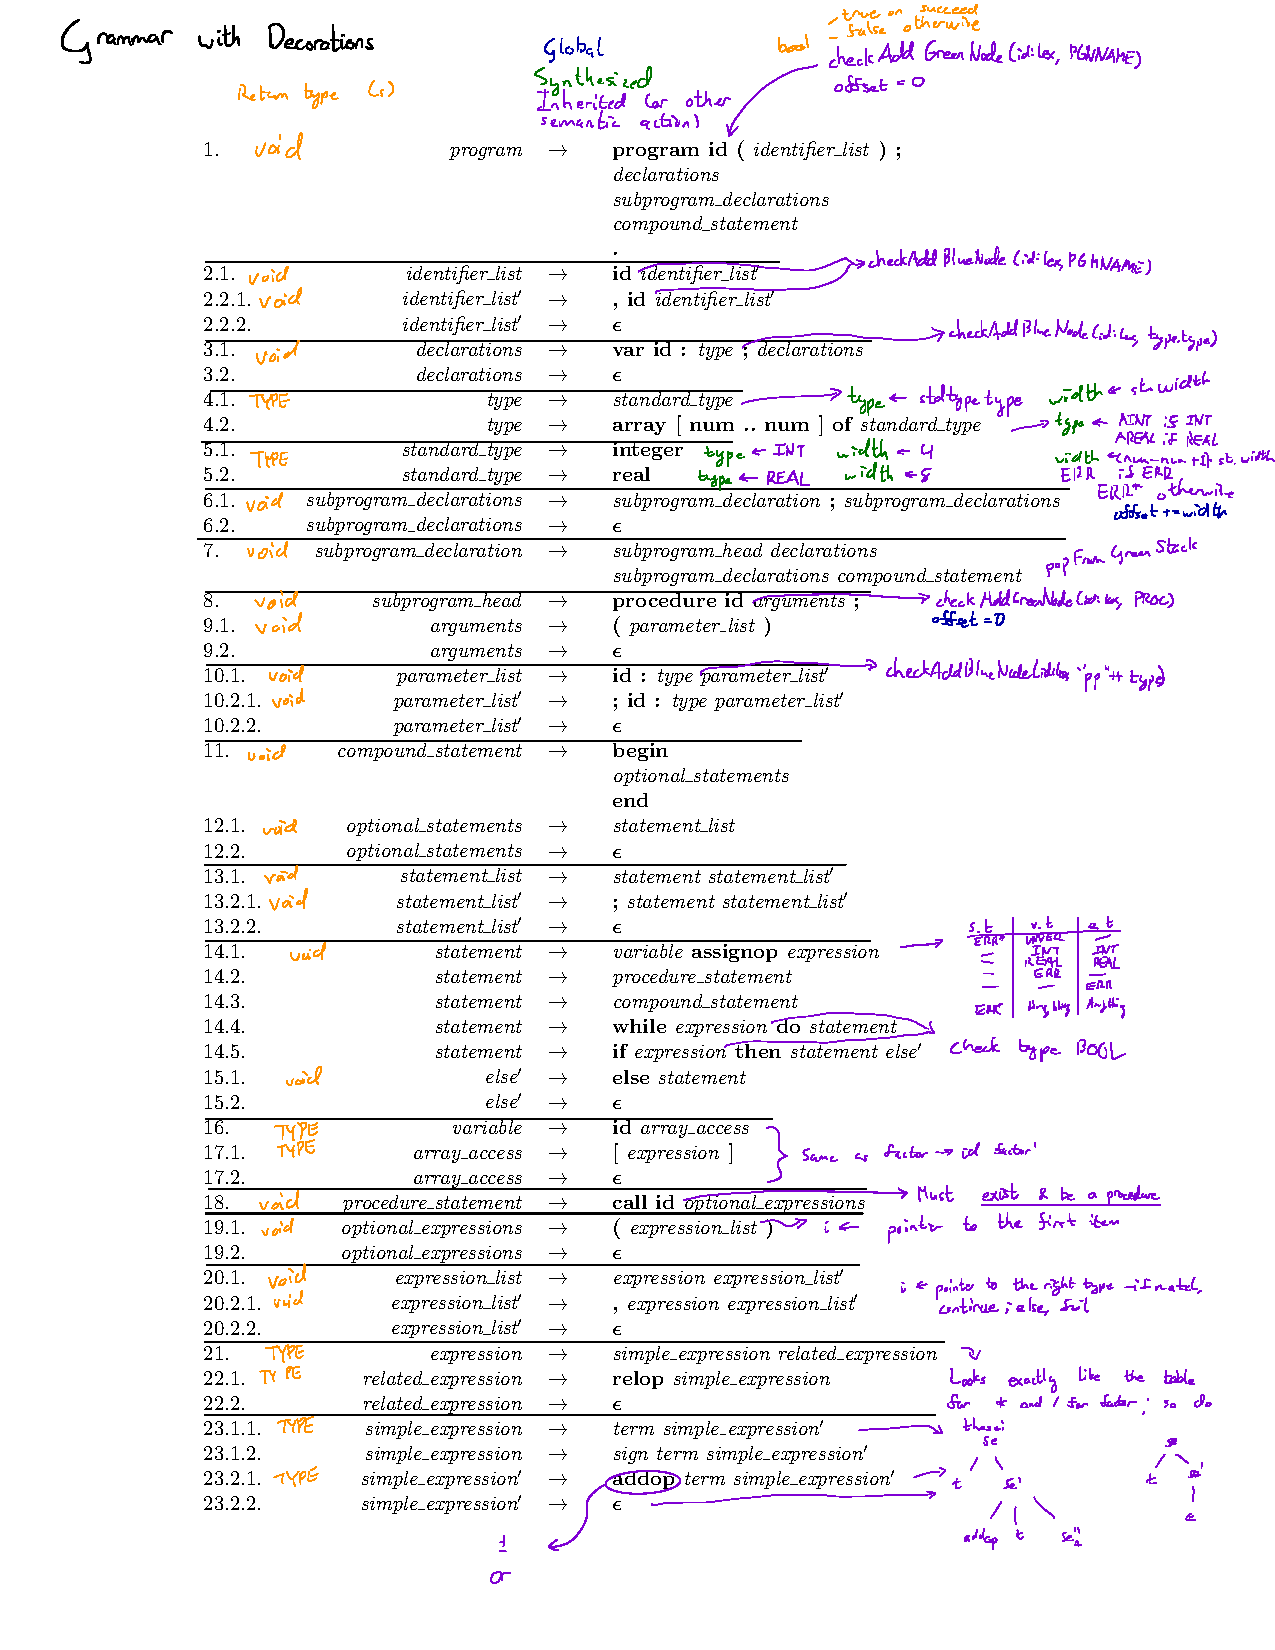
\includepdf[pages=-]{grammar_steps/decorated.pdf}

    \section{Implementation}
    I merely modified the productions to enforce the rules, according to the
    decorated grammar given above.

    The declarations processing was interesting---I used a binary tree with
    left-child, right-sibling notation. I a pointer to the bottom of the
    tree at all times. Whenever anything was added to the tree, I updated
    the bottom pointer to point to the new data.
    Then, whenever a new scope was declared,
    I added a pointer to that tree node to the stack; whenever the new scope
    ended, I set the bottom pointer to the value popped from the stack, and
    set a flag to add to the right of the child.

    If any errors were encountered while parsing, the error is added
    to the error queue. Then, the error is printed before the next token
    is collected. In this situation, multiple semantic errors could happen
    on the same token, so I had to create a separate message for each one
    and add it to a queue.

    \section{Discussion \& Conclusions}
    Implementing this project definitely taught me about the importance
    of an $LL(1)$ grammar, and how neat the recursive descent parser is.
    Decorating the grammar is a really cool way of implementing the compiler.

    I wrote this compiler in C, with no external code of any kind. It was
    compiled with clang on macOS Sierra.

    \clearpage{}
    \section*{Appendix 1: Sample Inputs and Outputs} % Input and output files.
    \subsection{Error-Filled}
    \ShowSampleFile{appendix1/error_full/error_full.pas}{Error-Full Source Code}
    \ShowSampleFile{appendix1/error_full/listing.txt}{Error-Full Listing File}
    \ShowSampleFile{appendix1/error_full/mem.txt}{Error-Full Semantic Mem File}
    \ShowTokenFile{appendix1/error_full/tokens.dat}{Error-Full Token File}

    \clearpage{}
    \subsection{Just Semantic Errors}
    \ShowSampleFile{appendix1/just_sem/debug.pas}{Just Semantic Source Code}
    \ShowSampleFile{appendix1/just_sem/listing.txt}{Just Semantic Listing File}
    \ShowSampleFile{appendix1/just_sem/mem.txt}{Just Semantic Mem File}
    \ShowTokenFile{appendix1/just_sem/tokens.dat}{Just Semantic Token File}

    \clearpage{}
    \subsection{Error-Free}
    \ShowSampleFile{appendix1/error_free/error_test.pas}{Error-Free Source Code}
    \ShowSampleFile{appendix1/error_free/listing.txt}{Error-Free Listing File}
    \ShowSampleFile{appendix1/error_free/mem.txt}{Error-Free Mem File}
    \ShowTokenFile{appendix1/error_free/tokens.dat}{Error-Free Token File}

    \twocolumn{}
    \section*{Appendix 2: Program Listings}
    \ShowSourceFile{code/compiler.c}{compiler.c}
    \ShowSourceFile{code/dataStructures/declarationsTree/declarationsTree.h}{declarationsTree.h}
    \ShowSourceFile{code/dataStructures/linkedList/linkedlist.h}{linkedlist.h}
    \ShowSourceFile{code/errorHandler/errorHandler.h}{errorHandler.h}
    \ShowSourceFile{code/globals/globals.h}{globals.h}
    \ShowSourceFile{code/handler/handler.h}{handler.h}
    \ShowSourceFile{code/parser/parser.h}{parser.h}
    \ShowSourceFile{code/parser/productions/productions.h}{productions.h}
    \ShowSourceFile{code/symbolTable/symbolTable.h}{symbolTable.h}
    \ShowSourceFile{code/tokenizer/machines/machines.h}{machines.h}
    \ShowSourceFile{code/tokenizer/tokenizer.h}{tokenizer.h}
    \ShowSourceFile{code/tokenizer/tokens.h}{tokens.h}
    \ShowSourceFile{code/dataStructures/declarationsTree/declarationsTree.c}{declarationsTree.c}
    \ShowSourceFile{code/dataStructures/linkedList/linkedlist.c}{linkedlist.c}
    \ShowSourceFile{code/errorHandler/errorHandler.c}{errorHandler.c}
    \ShowSourceFile{code/globals/globals.c}{globals.c}
    \ShowSourceFile{code/handler/handler.c}{handler.c}
    \ShowSourceFile{code/parser/parser.c}{parser.c}
    \ShowSourceFile{code/parser/productions/arguments.c}{arguments.c}
    \ShowSourceFile{code/parser/productions/array_access.c}{array_access.c}
    \ShowSourceFile{code/parser/productions/compound_statement.c}{compound_statement.c}
    \ShowSourceFile{code/parser/productions/declarations.c}{declarations.c}
    \ShowSourceFile{code/parser/productions/else_tail.c}{else_tail.c}
    \ShowSourceFile{code/parser/productions/expression.c}{expression.c}
    \ShowSourceFile{code/parser/productions/expression_list.c}{expression_list.c}
    \ShowSourceFile{code/parser/productions/expression_list_tail.c}{expression_list_tail.c}
    \ShowSourceFile{code/parser/productions/factor.c}{factor.c}
    \ShowSourceFile{code/parser/productions/factor_tail.c}{factor_tail.c}
    \ShowSourceFile{code/parser/productions/id_list.c}{id_list.c}
    \ShowSourceFile{code/parser/productions/id_list_tail.c}{id_list_tail.c}
    \ShowSourceFile{code/parser/productions/optional_expressions.c}{optional_expressions.c}
    \ShowSourceFile{code/parser/productions/optional_statements.c}{optional_statements.c}
    \ShowSourceFile{code/parser/productions/parameter_list.c}{parameter_list.c}
    \ShowSourceFile{code/parser/productions/parameter_list_tail.c}{parameter_list_tail.c}
    \ShowSourceFile{code/parser/productions/procedure_statement.c}{procedure_statement.c}
    \ShowSourceFile{code/parser/productions/program.c}{program.c}
    \ShowSourceFile{code/parser/productions/related_expression.c}{related_expression.c}
    \ShowSourceFile{code/parser/productions/sign.c}{sign.c}
    \ShowSourceFile{code/parser/productions/simple_expression.c}{simple_expression.c}
    \ShowSourceFile{code/parser/productions/simple_expression_tail.c}{simple_expression_tail.c}
    \ShowSourceFile{code/parser/productions/standard_type.c}{standard_type.c}
    \ShowSourceFile{code/parser/productions/statement.c}{statement.c}
    \ShowSourceFile{code/parser/productions/statement_list.c}{statement_list.c}
    \ShowSourceFile{code/parser/productions/statement_list_tail.c}{statement_list_tail.c}
    \ShowSourceFile{code/parser/productions/subprogram_declaration.c}{subprogram_declaration.c}
    \ShowSourceFile{code/parser/productions/subprogram_declarations.c}{subprogram_declarations.c}
    \ShowSourceFile{code/parser/productions/subprogram_head.c}{subprogram_head.c}
    \ShowSourceFile{code/parser/productions/term.c}{term.c}
    \ShowSourceFile{code/parser/productions/term_tail.c}{term_tail.c}
    \ShowSourceFile{code/parser/productions/type.c}{type.c}
    \ShowSourceFile{code/parser/productions/variable.c}{variable.c}
    \ShowSourceFile{code/symbolTable/symbolTable.c}{symbolTable.c}
    \ShowSourceFile{code/tokenizer/machines/addop.c}{addop.c}
    \ShowSourceFile{code/tokenizer/machines/catchall.c}{catchall.c}
    \ShowSourceFile{code/tokenizer/machines/grouping.c}{grouping.c}
    \ShowSourceFile{code/tokenizer/machines/idres.c}{idres.c}
    \ShowSourceFile{code/tokenizer/machines/mulop.c}{mulop.c}
    \ShowSourceFile{code/tokenizer/machines/numbers.c}{numbers.c}
    \ShowSourceFile{code/tokenizer/machines/relop.c}{relop.c}
    \ShowSourceFile{code/tokenizer/machines/whitespace.c}{whitespace.c}
    \ShowSourceFile{code/tokenizer/tokenizer.c}{tokenizer.c}
    \ShowSourceFile{code/tokenizer/tokens.c}{tokens.c}

\end{document}
